% ============================================================
%  NotebookBuildAudit-Presentation
%  Beamer presentation for internal / team audience
%  Based on NotebookBuildAudit-Complete.tex
%  + ROBIN-HOOD & Metanym Game concepts integrated
%  Compile with: pdflatex (twice) or latexmk -pdf
% ============================================================
\documentclass[11pt, aspectratio=169]{beamer}

% ── Theme ──────────────────────────────────────────────────
\usetheme[numbering=fraction, block=fill]{metropolis}
\usecolortheme{spruce}
\setbeamertemplate{items}[circle]

% ── Packages ───────────────────────────────────────────────
\usepackage[T1]{fontenc}
\usepackage[utf8]{inputenc}
\usepackage{booktabs}
\usepackage{tabularx}
\usepackage{xcolor}
\usepackage{listings}
\usepackage{tikz}
\usetikzlibrary{shapes.geometric, arrows.meta, positioning, calc}
\usepackage{forest}
\usepackage{amsmath}

% ── Column types ───────────────────────────────────────────
\newcolumntype{Y}{>{\raggedright\arraybackslash}X}

% ── Forest style ───────────────────────────────────────────
\forestset{
  mono tree/.style={
    for tree={
      calign=center,
      l sep=6mm,
      s sep=4mm,
      inner sep=4pt,
      draw,
      rounded corners=2pt,
      line width=0.3pt,
      font=\small\sffamily,
      text width=2.8cm,
      align=center,
    }
  }
}

% ── Colours ────────────────────────────────────────────────
\definecolor{tealFill}{HTML}{9FE1CB}
\definecolor{tealStroke}{HTML}{0F6E56}
\definecolor{tealTxt}{HTML}{04342C}
\definecolor{purpleFill}{HTML}{CECBF6}
\definecolor{purpleStroke}{HTML}{534AB7}
\definecolor{purpleTxt}{HTML}{26215C}
\definecolor{coralFill}{HTML}{F5C4B3}
\definecolor{coralStroke}{HTML}{993C1D}
\definecolor{coralTxt}{HTML}{4A1B0C}
\definecolor{grayFill}{HTML}{D3D1C7}
\definecolor{grayStroke}{HTML}{888780}

% ── TikZ styles ────────────────────────────────────────────
\tikzset{
  base/.style={
    rectangle, rounded corners=4pt,
    text width=3.2cm, align=center,
    minimum height=0.9cm,
    inner sep=5pt,
    draw, line width=0.4pt,
    font=\small
  },
  teal/.style={base, fill=tealFill, draw=tealStroke, text=tealTxt},
  purple/.style={base, fill=purpleFill, draw=purpleStroke, text=purpleTxt},
  coral/.style={base, fill=coralFill, draw=coralStroke, text=coralTxt},
  gray/.style={base, fill=grayFill, draw=grayStroke},
}

% ── Title info ─────────────────────────────────────────────
\title{Notebook Build Audit \\ \& Execution System}
\subtitle{Construction, Audit, and Intelligent LLM Evaluation}
\date{}

\begin{document}

% ============================================================
\maketitle
% ============================================================

% ============================================================
\begin{frame}{The Challenge}
  \textbf{Computational notebooks (Jupyter) are the dominant medium for DS/ML --- but they introduce systemic risks:}

  \vspace{0.4cm}
  \begin{itemize}
    \item \alert{Untrusted execution} --- notebooks from collaborators, open-source, or AI
      assistants without deterministic safety guarantees

    \item \alert{Lack of deterministic builds} --- ad hoc environment pinning, missing
      dependencies, absent seed controls $\rightarrow$ different results across machines

    \item \alert{No structured audit protocol} --- no systematic methodology for reviewing
      notebooks before production, publication, or merge
  \end{itemize}

  \vspace{0.5cm}
  \begin{quote}
    ``Existing code review practices are insufficient for the unique failure modes of
    notebook-based ML pipelines.''
  \end{quote}
\end{frame}

% ============================================================
\begin{frame}{Two Complementary Frameworks}
  \centering
  \vspace{0.3cm}

  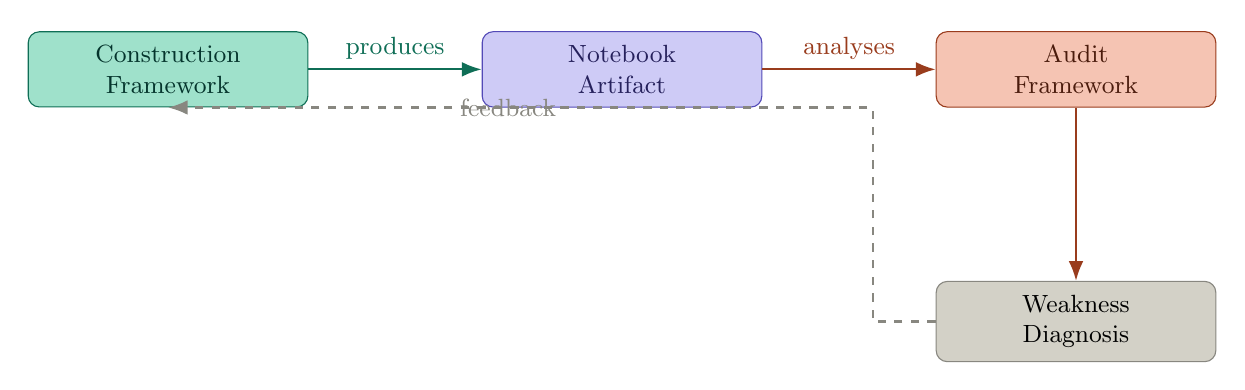
\begin{tikzpicture}[node distance=2.2cm]
    \node[teal] (construction) {Construction\\Framework};
    \node[purple, right=of construction] (artifact) {Notebook\\Artifact};
    \node[coral, right=of artifact] (audit) {Audit\\Framework};
    \node[gray, below=of audit] (findings) {Weakness\\Diagnosis};

    \draw[-{Latex[length=2.5mm]}, tealStroke, thick]
      (construction) -- node[above] {\small produces} (artifact);
    \draw[-{Latex[length=2.5mm]}, coralStroke, thick]
      (artifact) -- node[above] {\small analyses} (audit);
    \draw[-{Latex[length=2.5mm]}, coralStroke, thick]
      (audit) -- (findings);
    \draw[-{Latex[length=2.5mm]}, grayStroke, thick, dashed]
      (findings.west) -- ++(-0.8,0) |- (construction.south)
      node[pos=0.8, right] {\small feedback};
  \end{tikzpicture}

  {\footnotesize
  \vspace{0.1cm}
  \begin{description}
    \item[Construction Framework] \hfill \\
      \textit{Forward-looking} --- guides the author to produce a reproducible,
      well-structured notebook from the ground up.

    \item[Audit Framework] \hfill \\
      \textit{Backward-looking} --- systematically assesses quality, correctness,
      and risk of an existing notebook.
  \end{description}
  }
\end{frame}

% ============================================================
\begin{frame}{Construction Framework --- Three Phases}
  \centering
  \vspace{-0.3cm}
  \resizebox{0.75\textwidth}{!}{%
    \begin{forest}
      mono tree,
      [Notebook Construction\\Strategy
        [Modular\\Section Design]
        [{Reproducibility Standards\\(seeds, environments)}]
        [Narrative Documentation\\Guidelines]
        [Output Artifact\\Management]
      ]
    \end{forest}
  }

  \vspace{0.1cm}
  \begin{columns}[T]
    \column{0.33\textwidth}
      \textbf{Phase 1 --- Scaffold}
      \begin{itemize}\scriptsize
        \item Single responsibility
        \item 8 canonical section headers
        \item Pin environment upfront
        \item Global reproducibility controls
      \end{itemize}

    \column{0.33\textwidth}
      \textbf{Phase 2 --- Write}
      \begin{itemize}\scriptsize
        \item One section at a time
        \item Markdown intent per code cell
        \item Explicit variable passing
        \item Three-block refactor threshold
      \end{itemize}

    \column{0.33\textwidth}
      \textbf{Phase 3 --- Validate}
      \begin{itemize}\scriptsize
        \item Restart kernel per section
        \item Cell idempotency check
        \item Linear execution order
        \item Versioned artifact routing
      \end{itemize}
  \end{columns}
\end{frame}

% ============================================================
\begin{frame}{LLM-as-a-Judge --- Two Evaluation Layers}
  \textbf{Why LLM-based evaluation?} Notebook auditing combines \alert{objective} and
  \alert{subjective} tasks.

  \vspace{0.25cm}
  \begin{columns}[T]
    \column{0.48\textwidth}
      \textbf{Layer 1 --- Deterministic}
      \begin{itemize}\small
        \item Dependency validation
        \item Execution reproducibility
        \item Train/test split verification
        \item Artifact existence
      \end{itemize}
      \vspace{0.1cm}
      {\small\textit{Binary, reproducible --- programmatic checks}}

    \column{0.48\textwidth}
      \textbf{Layer 2 --- LLM Judge}
      \begin{itemize}\small
        \item Documentation quality
        \item Conceptual coherence
        \item Methodological soundness
        \item Deployment readiness
      \end{itemize}
      \vspace{0.1cm}
      {\small\textit{Semantic reasoning --- structured evaluation prompts}}
  \end{columns}

  \vspace{0.3cm}
  \textbf{Key insight:} Decompose evaluation into explicit criteria (G-Eval).
  Known biases: position, verbosity, self-enhancement.
\end{frame}

% ============================================================
\begin{frame}{ROBIN-HOOD --- The Algorithm}
  \textbf{Paper:} Saha, Wagde \& Kveton (2026) --- \textit{LLM-as-Judge on a Budget}

  \vspace{0.1cm}
  \textbf{Problem:} $K$ items, budget $B$ queries --- how to allocate to minimise error?

  \vspace{0.1cm}
  \textbf{Key insight:} \alert{High-variance} items need more queries; stable items need fewer.

  \vspace{0.1cm}
  \begin{columns}[T]
    \column{0.48\textwidth}
      \textbf{Algorithm (adaptive):}
      \begin{enumerate}\footnotesize
        \item Evaluate every item once
        \item Compute $\mu_i$ and variance $\sigma^2_i$ per item
        \item Next query $\rightarrow$ $\arg\max_i \sigma^2_i / n_i$
        \item Repeat until budget exhausted
      \end{enumerate}

    \column{0.48\textwidth}
      \textbf{Theoretical guarantee:}
      \[
      \tilde{O}\!\left(\sqrt{\frac{\textstyle\sum_{i=1}^K \sigma_i^2}{B}}\right)
      \]
      \begin{itemize}\footnotesize
        \item Same accuracy at \alert{half the budget}
        \item Tested on \textit{SFF} \& \textit{HelpSteer2}
      \end{itemize}
  \end{columns}

  \vspace{0.1cm}
  {\footnotesize\textit{``Leverages multi-armed bandit theory to dynamically
  concentrate queries where uncertainty is highest.''}}
\end{frame}

% ============================================================
\begin{frame}{ROBIN-HOOD --- Application to 6-Pass Audit}
  \centering
  Different passes have different variance profiles:

  \vspace{0.15cm}
  {\footnotesize
  \begin{tabularx}{\textwidth}{l l c}
    \toprule
    \textbf{Pass} & \textbf{Type} & \textbf{Allocation} \\
    \midrule
    1 --- Structural Overview      & Easy   & Low    \\
    2 --- Reproducibility Check    & Easy   & Low    \\
    3 --- Data Integrity Review    & Medium & Medium \\
    4 --- ML Correctness Audit     & Hard   & \alert{High} \\
    5 --- Code Quality Review      & Medium & Medium \\
    6 --- Deployment Readiness     & Hard   & High \\
    \bottomrule
  \end{tabularx}
  }

  \vspace{0.15cm}
  \textbf{Impact:} Dynamically allocates to Passes 4 \& 6 instead of uniform.
  Same precision, $\sim$\alert{50\% fewer queries}.

  \vspace{0.1cm}
  {\footnotesize\emph{``Unevaluated variance wastes budget. Measure it --- then allocate.''}}
\end{frame}

% ============================================================
\begin{frame}{The Metanym Game --- A Discovery}
  \textbf{Paper:} David Nordfors (2026) --- \textit{The Metanym Game}

  \vspace{0.15cm}
  \textbf{What is it?} A competitive word game where LLMs generate and
  evaluate analogies. No fixed test set --- contamination-resistant by design.

  \vspace{0.2cm}
  \begin{columns}[T]
    \column{0.48\textwidth}
      \textbf{SVD on the rating matrix}
      \vspace{0.1cm}
      \begin{itemize}\small
        \item $K$ models act as both generators and judges
        \item Build $K \times K$ rating matrix
        \item Singular Value Decomposition reveals latent skills
      \end{itemize}

    \column{0.48\textwidth}
      \textbf{Two key findings}
      \vspace{0.1cm}
      \begin{itemize}\small
        \item[1.] Factual correlation with GPQA Diamond:
          $\mathbf{r = 0.92}$
          (no ground truth needed)
        \item[2.] \alert{Generating $\boldsymbol{\neq}$ Evaluating}
          --- dissociated skills
      \end{itemize}
  \end{columns}

  \vspace{0.2cm}
  \begin{alertblock}{Dissociation finding}
    The best generators are middling judges. The sharpest judge is a mid-pack
    generator. \textbf{Never assume the same model excels at both tasks.}
  \end{alertblock}
\end{frame}

% ============================================================
\begin{frame}{Multi-Judge Budget Allocation}
  \textbf{Paper 2:} \textit{Instance-Optimal Estimation with Multiple LLM Judges on a Budget}

  \vspace{0.1cm}
  Extends ROBIN-HOOD: multiple judges available, each with \alert{different cost \& accuracy}.

  \vspace{0.1cm}
  \begin{columns}[T]
    \column{0.48\textwidth}
      \textbf{Decision space doubles:}
      \begin{itemize}\footnotesize
        \item \textbf{Which items} to evaluate
        \item \textbf{Which judge} for each query
      \end{itemize}
      \vspace{0.1cm}
      \textbf{Rule of thumb:}
      \begin{itemize}\footnotesize
        \item Cheap judges for easy items
        \item Expensive judges for hard items
        \item Repeat only when uncertainty is high
      \end{itemize}

    \column{0.48\textwidth}
      \textbf{Theoretical result:}
      \begin{itemize}\footnotesize
        \item \alert{Instance-optimal}: no strategy achieves
          lower error with same budget
        \item One right judge per item can beat
          combining multiple on every item
      \end{itemize}
      \vspace{0.1cm}
      \textbf{Practical:} GPT-5 for hard passes, Gemini-2.5 for
      routine, small local model for trivial ones.
  \end{columns}
\end{frame}

% ============================================================
\begin{frame}{Panel Architecture --- Implementing the Findings}
  \centering
  Both papers conclude: \textbf{a panel of diverse judges, not a single LLM.}

  \vspace{0.15cm}
  {\footnotesize
  \begin{tabularx}{\textwidth}{X X}
    \toprule
    \textbf{ROBIN-HOOD says} & \textbf{Metanym Game says} \\
    \midrule
    Allocate budget by variance & Use diverse models \\
    Concentrate on hard items   & Gen $\neq$ Evaluators \\
    Same accuracy, half cost    & Panels beat individuals \\
    \bottomrule
  \end{tabularx}
  }

  \vspace{0.15cm}
  \begin{columns}[T]
    \column{0.45\textwidth}
      \begin{block}{Scheduler (ROBIN-HOOD)}
        \begin{itemize}\footnotesize
          \item Tracks variance per audit pass
          \item Decides \textbf{how many} queries
        \end{itemize}
      \end{block}

    \column{0.45\textwidth}
      \begin{block}{Panel (Metanym-inspired)}
        \begin{itemize}\footnotesize
          \item GPT-5, Claude, Gemini, Llama, Mistral
          \item Decides \textbf{which model} per query
          \item SVD tracks competence over time
        \end{itemize}
      \end{block}
  \end{columns}

  \vspace{0.1cm}
  {\footnotesize\textit{ROBIN-HOOD decides quantity; Panel decides quality.}}
\end{frame}

% ============================================================
\begin{frame}{Prompt Crafting --- Three-Level Structure}
  \centering
  \vspace{-0.1cm}

  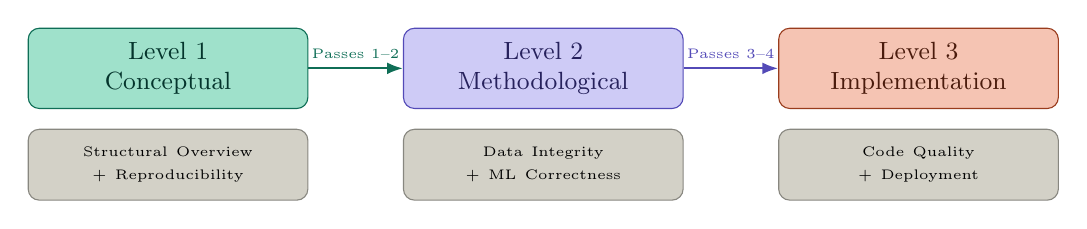
\begin{tikzpicture}[node distance=1.2cm]
    \node[teal] (l1) {Level 1\\Conceptual};
    \node[purple, right=of l1] (l2) {Level 2\\Methodological};
    \node[coral, right=of l2] (l3) {Level 3\\Implementation};

    \draw[-{Latex[length=2mm]}, tealStroke, thick]
      (l1) -- node[above] {\tiny Passes 1--2} (l2);
    \draw[-{Latex[length=2mm]}, purpleStroke, thick]
      (l2) -- node[above] {\tiny Passes 3--4} (l3);

    \node[gray, below=0.25cm of l1] (g1) {\tiny Structural Overview\\[-0.1cm] + Reproducibility};
    \node[gray, below=0.25cm of l2] (g2) {\tiny Data Integrity\\[-0.1cm] + ML Correctness};
    \node[gray, below=0.25cm of l3] (g3) {\tiny Code Quality\\[-0.1cm] + Deployment};
  \end{tikzpicture}

  \vspace{0.1cm}
  \begin{columns}[T]
    \column{0.32\textwidth}
      \begin{block}{Gate 1 $\rightarrow$ 2}
        \footnotesize Notebook fails end-to-end? Flag or proceed.
      \end{block}

    \column{0.32\textwidth}
      \begin{block}{Gate 2 $\rightarrow$ 3}
        \footnotesize Methodological flaws (leakage, invalid CV)? Halt with caveats.
      \end{block}

    \column{0.32\textwidth}
      \begin{block}{After Level 3}
        \footnotesize Final report: risk scores across 6 passes, recommendations.
      \end{block}
  \end{columns}
\end{frame}

% ============================================================
\begin{frame}{Six-Pass Audit Protocol}
  \centering
  \vspace{-0.2cm}
  \resizebox{0.8\textwidth}{!}{%
    \begin{forest}
      mono tree,
      [Notebook Audit\\Strategy
        [{Multi-Pass Incremental\\Analysis}]
        [Hierarchical\\Review Depth]
        [Pattern Summarization\\with Thresholds]
        [{User-Guided Focus Areas\\(AI-assisted context)}]
      ]
    \end{forest}
  }

  \vspace{0.1cm}
  \begin{columns}[T]
    \column{0.33\textwidth}
      \textbf{Level 1 --- Conceptual}
      \begin{enumerate}\scriptsize
        \item \textbf{Pass 1} --- Structural Overview
        \item \textbf{Pass 2} --- Reproducibility Check
      \end{enumerate}
      \scriptsize\textit{Deliverables:} Section map, red flags

    \column{0.33\textwidth}
      \textbf{Level 2 --- Methodological}
      \begin{enumerate}\scriptsize
        \setcounter{enumi}{2}
        \item \textbf{Pass 3} --- Data Integrity Review
        \item \textbf{Pass 4} --- ML Correctness Audit
      \end{enumerate}
      \scriptsize\textit{Deliverables:} Pipeline report, checklist

    \column{0.33\textwidth}
      \textbf{Level 3 --- Implementation}
      \begin{enumerate}\scriptsize
        \setcounter{enumi}{4}
        \item \textbf{Pass 5} --- Code Quality Review
        \item \textbf{Pass 6} --- Deployment Readiness
      \end{enumerate}
      \scriptsize\textit{Deliverables:} Smell report, readiness score
  \end{columns}
\end{frame}

% ============================================================
\begin{frame}{Architecture Overview}
  \centering
  \vspace{-0.2cm}
  {\footnotesize
  \begin{columns}[T]
    \column{0.45\textwidth}
      \textbf{Concept}
      \begin{itemize}
        \item Construction $\leftrightarrow$ Audit lifecycle
        \item Three-level audit with HITL gates
        \item Provider-agnostic LLM layer
      \end{itemize}
      \vspace{0.3cm}
      \textbf{Physical}
      \begin{itemize}
        \item Docker Compose (5 services)
        \item Ephemeral sandbox per notebook audit
        \item Local or cloud (Ollama/OpenAI)
      \end{itemize}

    \column{0.50\textwidth}
      \textbf{Logical}
      \begin{itemize}
        \item React + TypeScript Dashboard
        \item FastAPI REST + SSE Gateway
        \item \alert{ROBIN-HOOD Scheduler}
        \item \alert{LLM Panel Proxy} (Strategy Pattern)
        \item Audit State Machine
        \item @jupyter-kit Execution Engine
        \item PostgreSQL + SQLAlchemy
      \end{itemize}
  \end{columns}
  }
\end{frame}

% ============================================================
\begin{frame}{Cost Analysis and ROI}
  \centering
  \textbf{Monthly inference cost --- 10,000 item evaluations}

  \vspace{0.15cm}
  {\footnotesize
  \begin{tabularx}{0.7\textwidth}{l r r}
    \toprule
    \textbf{Approach} & \textbf{Queries} & \textbf{Monthly cost} \\
    \midrule
    Uniform (5 each)      & 50,000 & \$1,500 \\
    Uniform (1 each)      & 10,000 & \$300 (poor) \\
    \textbf{ROBIN-HOOD}   & $\sim$15,000 & $\sim$\$450 \\
    \textbf{ROBIN-HOOD + Panel} & $\sim$12,000 & $\sim$\$350 \\
    \bottomrule
  \end{tabularx}
  }

  \vspace{0.15cm}
  {\footnotesize
  \begin{tabularx}{0.9\textwidth}{l r r r}
    \toprule
    \textbf{Period} & \textbf{Without} & \textbf{With ROBIN} & \textbf{Savings} \\
    \midrule
    Month 1 & \$1,500 & \$1,000 + \$500 dev & \$0 \\
    Month 2 & \$1,500 & \$450 & \alert{\$1,050} \\
    \textbf{Annual} & \textbf{\$18,000} & \textbf{\$11,400} & \textbf{\$6,600} \\
    \bottomrule
  \end{tabularx}
  }

  \vspace{0.1cm}
  {\small\textbf{ROI:} 37\% year 1, $\sim$70\% year 2+.
   At 100K items/month: $\sim$\$10K/month savings.}
\end{frame}

% ============================================================
\begin{frame}{LLMOps Pipeline}
  \centering
  How ROBIN-HOOD + Metanym Game integrate into continuous evaluation:

  \vspace{0.1cm}
  \footnotesize
  \begin{columns}[T]
    \column{0.48\textwidth}
      \begin{block}{Monitoring \& Observability}
        \begin{itemize}\scriptsize
          \item Cost per pass and per judge model
          \item Variance tracking per audit item
          \item Judge competence drift detection
        \end{itemize}
      \end{block}

      \vspace{0.1cm}
      \begin{block}{Feedback Loops}
        \begin{itemize}\scriptsize
          \item ROBIN-HOOD reallocates budget based on drift
          \item Panel rebalances as competence changes
          \item HITL triggers when variance exceeds threshold
          \item Periodic SVD recalibration
        \end{itemize}
      \end{block}

    \column{0.48\textwidth}
      \begin{block}{CI/CD Integration}
        \begin{itemize}\scriptsize
          \item New model $\rightarrow$ automatic evaluation by panel
          \item Competence score $\rightarrow$ deploy / reject
          \item Score drops $\rightarrow$ rollback + alert
        \end{itemize}
      \end{block}

      \vspace{0.1cm}
      \begin{block}{Key Metrics Dashboard}
        \begin{itemize}\scriptsize
          \item Query budget spent per pass
          \item Variance reduction over time
          \item Judge panel accuracy matrix
          \item Cost: ROBIN vs uniform
        \end{itemize}
      \end{block}
  \end{columns}
\end{frame}

% ============================================================
\begin{frame}{Papers Comparison}
  \centering
  \textbf{Three papers, one unified strategy}

  \vspace{0.15cm}
  {\footnotesize
  \begin{tabularx}{\textwidth}{l c c c}
    \toprule
    \textbf{Aspect} & \textbf{ROBIN-HOOD} & \textbf{Multi-Judge} & \textbf{Metanym} \\
    \midrule
    Adaptive budget         & \checkmark & \checkmark & --- \\
    Single judge            & \checkmark & \checkmark & --- \\
    Multiple judges         & --- & \checkmark & \checkmark \\
    Different judge costs   & --- & \checkmark & --- \\
    Gen \& Eval dissociation & --- & --- & \checkmark \\
    Optimality guarantee    & Partial & \checkmark & --- \\
    Panel architecture      & --- & Implied & \checkmark \\
    \bottomrule
  \end{tabularx}
  }

  \vspace{0.1cm}
  \begin{block}{Unified takeaway}
    \footnotesize\textbf{ROBIN-HOOD} $\to$ quantity. \textbf{Multi-Judge} $\to$ model.
    \textbf{Metanym} $\to$ diverse panel. Together: max precision, min cost.
  \end{block}
\end{frame}

% ============================================================
\begin{frame}{Resource Costs}
  \centering
  \begin{columns}[T]
    \column{0.48\textwidth}
      \textbf{Computational}
      \begin{table}\footnotesize
        \renewcommand{\arraystretch}{1.1}
        \begin{tabularx}{\textwidth}{l r}
          \toprule
          \textbf{Item} & \textbf{USD} \\
          \midrule
          Server PC & \$1{,}000 \\
          Hosting (3mo) & \$300 \\
          \midrule
          \textbf{Total Q1} & \textbf{\$1{,}300} \\
          \bottomrule
        \end{tabularx}
      \end{table}

      \vspace{0.05cm}
      \textbf{Development:} 8 weeks, 2 developers \hfill \textbf{Total:} \alert{\$5,000 USD}

    \column{0.48\textwidth}
      \textbf{Energetic --- Third Pillar Proposal}
      \begin{itemize}\footnotesize
        \item LLM inference is energy-intensive (0.01--0.1 kWh per pass)
        \item Notebook execution often wasteful
        \item ESG reporting increasingly required
      \end{itemize}

      \vspace{0.1cm}
      \textbf{Proposed compromise:}
      \begin{itemize}\footnotesize
        \item \textbf{Pass 7} (optional) --- Energy Impact Assessment
        \item Backends: RAPL, NVML, powermetrics
        \item Graceful degradation when unavailable
      \end{itemize}
  \end{columns}
\end{frame}

% ============================================================
\begin{frame}{Timeline \& Roadmap}
  \centering
  \renewcommand{\arraystretch}{1.3}
  \begin{tabularx}{\textwidth}{c Y c}
    \toprule
    \textbf{Phase} & \textbf{Summary} & \textbf{Duration} \\
    \midrule
    \textbf{1} &
    Dockerization, monorepo, sandbox spawning,
    dependency pinning &
    2 weeks \\

    \textbf{2} &
    FastAPI REST + SSE, \alert{ROBIN-HOOD Scheduler},
    \alert{LLM Panel Proxy}, Audit State Machine &
    3 weeks \\

    \textbf{3} &
    React dashboard, session management, live
    progress, risk visualisation &
    2 weeks \\

    \textbf{4} &
    E2E testing, \alert{panel competence tracking},
    security review, documentation &
    1 week \\
    \bottomrule
  \end{tabularx}

  \vspace{0.5cm}
  \textbf{Total: 8 weeks} --- 2 developers
\end{frame}

% ============================================================
\begin{frame}{Discussion Points}
  \centering
  \Large\textbf{What do we build first?}

  \vspace{0.3cm}
  {\footnotesize
  \begin{columns}[T]
    \column{0.45\textwidth}
      \begin{block}{Provider Strategy}
        \begin{itemize}
          \item Local (Ollama) vs cloud (OpenAI) as default?
          \item Offline-first or hybrid?
        \end{itemize}
      \end{block}

      \vspace{0.2cm}
      \begin{block}{Pass 7 Energy}
        \begin{itemize}
          \item Include from Phase 2 as experimental?
          \item Defer to Phase 4?
        \end{itemize}
      \end{block}

    \column{0.45\textwidth}
      \begin{block}{Scope}
        \begin{itemize}
          \item Full 6-pass from day one?
          \item Start with Level 1 only?
        \end{itemize}
      \end{block}

      \vspace{0.2cm}
      \begin{block}{Audience}
        \begin{itemize}
          \item Internal team only, or client-ready?
          \item Academic publication use case?
        \end{itemize}
      \end{block}
  \end{columns}
  }
\end{frame}

% ============================================================
\begin{frame}{Summary}
  \centering
  \Large\textbf{Notebook Build Audit \& Execution System}

  \vspace{0.5cm}
  \begin{columns}[T]
    \column{0.20\textwidth}
      \centering
      \textbf{Construction}\\
      {\small Build right.\\
      3 phases, 8 sections.}

    \column{0.20\textwidth}
      \centering
      \textbf{Audit}\\
      {\small Review any notebook.\\
      6 passes, 3 levels.}

    \column{0.20\textwidth}
      \centering
      \textbf{ROBIN-HOOD}\\
      {\small Budget allocation.\\
      Half the cost.}

    \column{0.20\textwidth}
      \centering
      \textbf{Panel}\\
      {\small Diverse judges.\\
      Gen $\neq$ Evaluate.}

    \column{0.20\textwidth}
      \centering
      \textbf{Resource}\\
      {\small Track energy.\\
      Optional Pass 7.}
  \end{columns}

  \vspace{0.8cm}
  {\Large\alert{Codificar experiencia humana, validar con supervisión sistemática.}}
\end{frame}

% ============================================================
\begin{frame}[allowframebreaks]{References}
  \footnotesize
  \begin{thebibliography}{9}

  \bibitem{saha2026robinhood}
  A.~Saha, A.~Wagde, and B.~Kveton,
  ``LLM-as-Judge on a Budget,''
  \textit{arXiv:2602.15481}, 2026.

  \bibitem{nordfors2026metanym}
  D.~Nordfors,
  ``The Metanym Game: A Self-Contained, Self-Consistent LLM Peer-Community
  Benchmark for Structural Intelligence,''
  \textit{arXiv:2606.21008}, 2026.

  \end{thebibliography}
\end{frame}

\end{document}
